\documentclass[conference]{IEEEtran}
\IEEEoverridecommandlockouts
\usepackage{cite}
\usepackage{amsmath,amssymb,amsfonts}
\usepackage{algorithmic}
\usepackage{graphicx}
\usepackage{booktabs}
\usepackage{textcomp}
\usepackage{xcolor}
\usepackage{tikz}
\usetikzlibrary{arrows.meta, positioning, fit, backgrounds, calc}
\def\BibTeX{{\rm B\kern-.05em{\sc i\kern-.025em b}\kern-.08em
    T\kern-.1667em\lower.7ex\hbox{E}\kern-.125emX}}
\begin{document}

\title{MANTIS Complete — A Unified Banking Multi-Agent Security, Compliance, and Observability Testbed

\thanks{Identify applicable funding agency here. If none, delete this.}
}

\author{\IEEEauthorblockN{1\textsuperscript{st} Given Name Surname}
\IEEEauthorblockA{\textit{dept. name of organization (of Aff.)} \\
\textit{name of organization (of Aff.)}\\
City, Country \\
email address or ORCID}
\and
\IEEEauthorblockN{2\textsuperscript{nd} Given Name Surname}
\IEEEauthorblockA{\textit{dept. name of organization (of Aff.)} \\
\textit{name of organization (of Aff.)}\\
City, Country \\
email address or ORCID}
\and
\IEEEauthorblockN{3\textsuperscript{rd} Given Name Surname}
\IEEEauthorblockA{\textit{dept. name of organization (of Aff.)} \\
\textit{name of organization (of Aff.)}\\
City, Country \\
email address or ORCID}
\and
\IEEEauthorblockN{4\textsuperscript{th} Given Name Surname}
\IEEEauthorblockA{\textit{dept. name of organization (of Aff.)} \\
\textit{name of organization (of Aff.)}\\
City, Country \\
email address or ORCID}
}

\maketitle

\begin{abstract}
MANTIS (Modular Agent Network Testbed for Instrumentation and Security) is a configuration-driven security, compliance, and observability testbed built directly on a real banking multi-agent system. This paper consolidates the system's two prior papers -- the original testbed~\cite{mantis_paper1} and its first set of post-paper extensions~\cite{mantis_paper2} -- into a single, complete account of MANTIS as it exists today, and adds one further extension neither prior paper covers: a toggleable Anti-Money Laundering (AML) office, ported from the legacy \texttt{Citi\_P3} codebase MANTIS itself was originally extracted from~\cite{citi_p3_repo}. The base system instruments an otherwise-unmodified front/mid/back-office banking agent system at five fixed control points (input, agent, interaction, tool, output) through a hook bus; an attack, failure, or defense plugin declares which point it targets entirely in YAML and is dispatched through the identical interface regardless of kind. Seven automated evaluator dimensions, a benchmarking suite that isolates instrumentation overhead from LLM sampling latency (median 0.19\% of run duration), and a reproducibility layer recording a configuration hash, seed, and full environment per run round out the base testbed. On top of this, MANTIS now ships: six security-mechanism plugins covering every category a defense-in-depth testbed should (amount guardrail, risk-aware routing guard with an optional compliant-route recovery mode, batch-integrity guard, response redaction, rate limiting, action isolation); four additional observability exporters (Jaeger, Grafana, Phoenix, Langfuse); three additional banking workloads (dispute filing, SAR/exception escalation, loan pre-approval) plus a second institution profile; a schema-driven minimal browser UI whose every mutating action shells out to the same CLI a terminal user would invoke; an extended scenario library of 19 measured baselines and 26 attack/fault variants; and a real, toggleable integration of the independently-developed Zero Trust Backplane project's signed Policy Decision Point. This paper's own new contribution is the \textbf{AML office}: a fourth, off-by-default banking domain carrying real structuring detection (sliding-window cumulative-deposit analysis), mule-ring detection (closed-loop graph traversal over a customer's transaction history), identity-document verification (Levenshtein name scoring), and an alert-lifecycle state machine (open~$\rightarrow$~in-investigation~$\rightarrow$~cleared/escalated-to-SAR), all ported with the detection logic itself unchanged from \texttt{Citi\_P3}, gated behind a dedicated \texttt{aml\_office:} toggle that leaves every existing configuration's root agent byte-identical when absent. Live verification against a real model across five new scenarios surfaced, and let us fix, two real integration defects before reporting the extension as working: a routing-instruction gap that silently misrouted an identity-verification request to the wrong banking domain entirely, and an alert-lifecycle capability that was fully implemented and unit-tested yet unreachable by any agent in the built tree. After both fixes, all five AML scenarios execute correctly against the live backend, including a persisted, re-read-and-confirmed database state change from a live agent's own tool call. The full offline test suite stands at 853 passing tests with neither optional dependency installed, 880 with both the Zero Trust and AML optional dependencies installed, zero failures in every combination.
\end{abstract}

\begin{IEEEkeywords}
multi-agent systems, adversarial security, large language models, banking, anti-money laundering, zero trust, observability, benchmarking
\end{IEEEkeywords}

\section{Introduction}

Large language model (LLM) agents are moving from single-turn assistants into orchestrated multi-agent systems that carry out multi-step business processes, and banking is a natural early target: recent work proposes multi-agent frameworks for financial anomaly detection \cite{anomaly_detection_finance} and credit assessment \cite{masca_credit}, each decomposing a task across specialized agents the way a bank already organizes front-, mid-, and back-office work. That same decomposition is also where new security risk enters -- inter-agent communication is an exploitable surface in its own right \cite{prompt_infection, aitm_communication_attacks}, and a broad survey of agentic security concludes most defenses evaluated in isolation can be bypassed by an adaptive attacker \cite{agentic_security_survey, security_considerations_mas}. No widely available testbed previously let a researcher take a realistic, domain-specific multi-agent system and run controlled adversarial experiments against it without either reimplementing the orchestration framework or editing the business logic under test \cite{redagentbench}.

This paper is a consolidation, not a third independent contribution. The original MANTIS paper~\cite{mantis_paper1} built the hook bus, the banking runtime adapter, five attack and failure configurations, a seven-dimension evaluator, and a benchmarking suite -- and named five extensions deliberately deferred to future work. A second paper~\cite{mantis_paper2} implemented all five: additional observability exporters, security-mechanism (defense) plugins, additional banking workloads and a second institution profile, a minimal schema-driven UI, and -- after a team decision reversed an earlier exclusion -- a real, toggleable integration of the independently-developed Zero Trust Backplane project~\cite{ztb_repo}. Both papers' own artifacts (code, tests, and recorded evidence) remain frozen and unmodified; this paper neither edits nor supersedes them, it reports the complete system built on top of them, plus one further extension neither of them covers.

That further extension is an \textbf{AML (Anti-Money Laundering) office}. MANTIS's banking agents were originally extracted from a larger legacy monorepo, \texttt{Citi\_P3}~\cite{citi_p3_repo}, during the first paper's own WP1 migration; that legacy codebase had a working AML investigation capability -- structuring detection, mule-ring detection, identity verification, SAR drafting, and alert triage -- that never made the transition into MANTIS's modular architecture. This paper ports it, deliberately following the same discipline the Zero Trust integration established: a real capability adapted into the existing architecture, not reimplemented from a specification, gated behind a toggle so every pre-existing configuration is unaffected, and verified against the live system's own emitted trace rather than accepted on a clean exit code. Section~\ref{sec:aml} reports that verification process finding two real integration defects before the extension could honestly be called complete, and the fixes for both.

The remainder of this paper is organized as follows. Section~\ref{sec:background} summarizes the motivation and related work established in~\cite{mantis_paper1}. Section~\ref{sec:architecture} describes the complete current architecture. Section~\ref{sec:attacks} summarizes the attack and failure plugin library and its live-verified evidence. Section~\ref{sec:defenses} summarizes the six security-mechanism plugins and the Zero Trust Backplane integration. Section~\ref{sec:aml} reports the AML office extension in full, the paper's own new contribution. Section~\ref{sec:workloads} summarizes additional banking workloads, institution profiles, the minimal UI, and the extended scenario library. Section~\ref{sec:evaluation} consolidates test and live-verification evidence for the complete system. Section~\ref{sec:conclusion} concludes.

\section{Background and Motivation}
\label{sec:background}

Multi-agent decomposition is a natural fit for banking because the workloads are already organized around specialized roles -- monitoring, investigation, compliance sign-off, decision -- and prior work demonstrates this pattern being actively explored in finance \cite{anomaly_detection_finance, masca_credit}. Three properties of multi-agent LLM systems create risk a single-agent deployment does not have: agents ingest content produced by \emph{other agents}, not only end users, so a compromised or spoofed agent's output can influence every downstream consumer \cite{prompt_infection}; routing and hand-off decisions are themselves attack surfaces, since an adversary who can intercept or relabel an inter-agent message can redirect a request to the wrong specialist or skip a required review step \cite{aitm_communication_attacks}; and tool invocation -- the mechanism by which an agent actually moves money or posts a ledger entry -- can be mutated in flight, a materially different threat than a model simply answering incorrectly. General red-teaming benchmarks for LLM agents \cite{redagentbench} provide reusable attack scaffolding but evaluate against synthetic or generic tasks rather than an existing, production-shaped business workflow, and are not designed around the constraint that the business logic under test must remain completely unmodified -- a constraint that matters because a testbed requiring edits to the fraud-review agent's own logic to add an experiment cannot be trusted to measure that agent's real behavior. Zero Trust architecture -- never trusting a request implicitly, mediating every action through explicit policy \cite{nist_zero_trust}, increasingly proposed specifically for agentic AI systems \cite{zero_trust_agentic_identity} -- is the complementary governance layer Section~\ref{sec:defenses} reports as a real, toggleable integration rather than the deliberately-deferred direction the first paper treated it as.

\section{Architecture}
\label{sec:architecture}

Figure~\ref{fig:architecture} shows the complete MANTIS pipeline as it stands today. An experiment is declared entirely in a YAML configuration; an orchestrator establishes a run identifier, seed, and lifecycle, then drives the banking workflow through a hook bus exposing five fixed control points -- input, agent, interaction, tool, and output. Each dispatch carries a typed context (run id, trace id, workflow id, stage, source, target, payload, metadata) to every registered plugin whose declared stages match; a plugin returns \emph{continue}, \emph{mutate}, \emph{skip}, \emph{deny}, \emph{delay}, or \emph{error}, and a mutation threads correctly to the next plugin in the same dispatch while the fact that one occurred is recorded in context metadata, so a plugin dispatched later in the same chain -- the observability plugin, by design, so it can observe every attack's effect -- can distinguish a genuinely adversarial event from an ordinary one. Beneath the hook bus, a banking runtime adapter presents one stable interface (\texttt{inventory()}, \texttt{workflows()}, \texttt{build()}) over four domains: front office (transaction monitoring, fraud detection, compliance, customer service, dispute filing), mid office (operations planning, representative assist, loan pre-approval), back office (end-of-day reconciliation, settlement, SAR/exception escalation), and -- new in this paper -- AML office (structuring/mule-ring/identity-document investigation and SAR drafting, Section~\ref{sec:aml}). The live inventory (\texttt{mantis --inventory}), introspected from the tool modules and agent registry rather than maintained as a hand-authored list, reports all four domains unconditionally -- 38 agents and 34 tools (33 banking-domain tools plus the underlying agent framework's own routing tool) -- since domain metadata registration is independent of any single run's configuration. The AML office's own toggle (Section~\ref{sec:aml}) is a separate, narrower axis: it governs only whether a \emph{given run}'s actual agent tree instantiates the AML office's 4 agents and 7 tools, not whether the inventory can discover or validate against them. Every run built without the toggle -- the only kind possible before this paper -- uses exactly the 34-agent, 27-tool front/mid/back-office tree the two prior papers describe.

\begin{figure}[t]
\centering
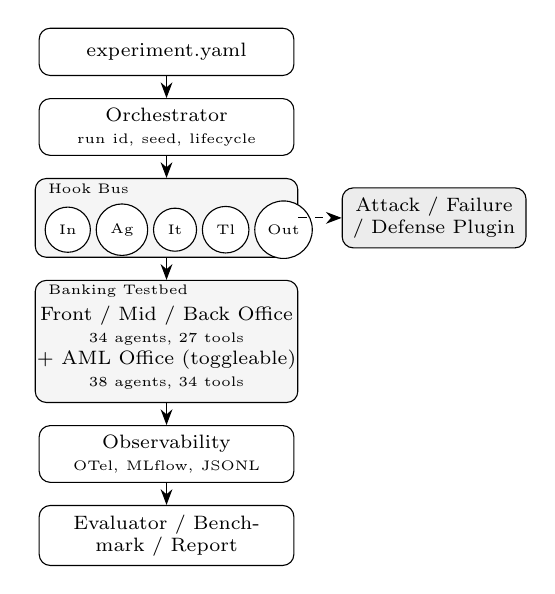
\begin{tikzpicture}[
    box/.style={draw, rounded corners, minimum height=0.6cm, text width=3.0cm, align=center, font=\scriptsize, fill=white},
    node distance=0.28cm,
    >={Stealth[length=2mm]}
]
\node[box] (cfg) {experiment.yaml};
\node[box, below=of cfg] (orch) {Orchestrator\\ \tiny run id, seed, lifecycle};
\node[draw, rounded corners, below=of orch, minimum height=1.0cm, text width=3.1cm, align=center, fill=gray!8] (hb) {};
\node[font=\tiny, above=0.05cm of hb.north west, anchor=north west, xshift=0.05cm] {Hook Bus};
\node[draw, circle, fill=white, font=\tiny, minimum size=0.42cm] (in) at ($(hb.west)+(0.42cm,-0.15cm)$) {In};
\node[draw, circle, fill=white, font=\tiny, minimum size=0.42cm, right=0.06cm of in] (ag) {Ag};
\node[draw, circle, fill=white, font=\tiny, minimum size=0.42cm, right=0.06cm of ag] (it) {It};
\node[draw, circle, fill=white, font=\tiny, minimum size=0.42cm, right=0.06cm of it] (tl) {Tl};
\node[draw, circle, fill=white, font=\tiny, minimum size=0.42cm, right=0.06cm of tl] (out) {Out};
\node[box, right=0.55cm of hb, fill=gray!15, text width=2.1cm] (atk) {Attack / Failure / Defense Plugin};
\node[draw, rounded corners, below=of hb, minimum height=1.55cm, text width=3.1cm, align=center, fill=gray!8] (bank) {};
\node[font=\tiny, above=0.06cm of bank.north west, anchor=north west, xshift=0.05cm] {Banking Testbed};
\node[font=\scriptsize, align=center] at ($(bank.center)+(0,-0.08cm)$) {Front / Mid / Back Office\\ \tiny 34 agents, 27 tools\\ + AML Office (toggleable)\\ \tiny 38 agents, 34 tools};
\node[box, below=of bank] (obs) {Observability\\ \tiny OTel, MLflow, JSONL};
\node[box, below=of obs] (eval) {Evaluator / Benchmark / Report};
\draw[->] (cfg) -- (orch);
\draw[->] (orch) -- (hb.north);
\draw[->, dashed] (hb.east) -- (atk.west);
\draw[->] (hb.south) -- (bank.north);
\draw[->] (bank.south) -- (obs.north);
\draw[->] (obs.south) -- (eval.north);
\end{tikzpicture}
\caption{The complete MANTIS pipeline. Every run passes through the same five-point hook bus regardless of banking domain; an attack, failure, or defense plugin attaches to the bus alongside the standard observability plugin. The AML office is a fourth banking domain, toggled per run, that does not change the pipeline shape when disabled.}
\label{fig:architecture}
\end{figure}

\begin{figure}[t]
\centering
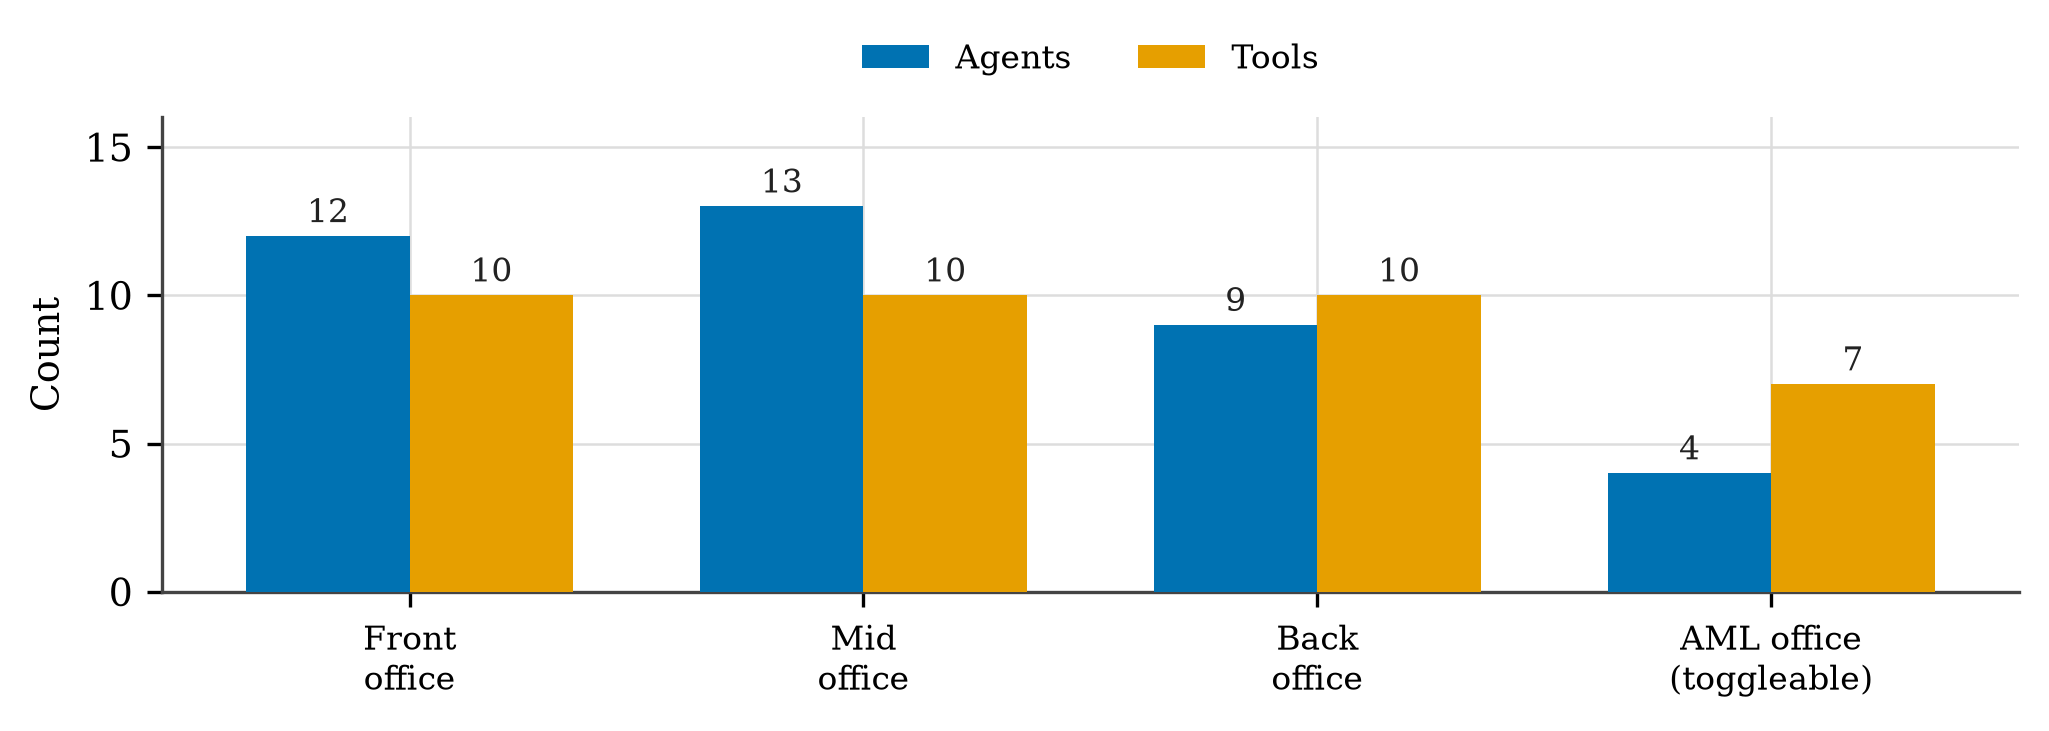
\includegraphics[width=\columnwidth]{figures/chart_domain_composition.png}
\caption{Agents and tools per banking domain (from the live \texttt{NativeBankingAdapter().inventory()}). The AML office is the only domain whose tool count exceeds its agent count -- most of its tools are read-only detection/lookup functions on a single investigator agent, rather than one tool per specialist agent as in the other three domains.}
\label{fig:domain-composition}
\end{figure}

Every hook dispatch is mapped to one of seven typed event families (experiment, workflow, agent, interaction, tool, security, evaluation), exported as portable JSONL, OpenTelemetry spans, and an MLflow run sharing the same configuration hash and seed, with four additional OTLP-compatible exporters (Jaeger, Grafana Tempo, Phoenix, Langfuse) added as one-line configuration changes that fail silently rather than aborting a run when no collector is reachable. An automated evaluator reads a run's trace and reports trace completeness, tool-use correctness, workflow outcome, hook-point coverage, banking-domain coverage, artifact integrity, and attack ground truth -- the last distinguishing a plugin that merely fired from one whose effect is corroborated against the configuration's own expected-tools/terminal-state baseline. Every run manifest records a SHA-256 configuration hash, the seed, the Python interpreter and dependency versions, the source commit, and -- newly tracked -- whether the run used a mock or live model and which model served it, so a reported result always traces back to the exact code, environment, and model that produced it.

\section{Attack and Failure Plugin Library}
\label{sec:attacks}

Five attack and failure configurations span all three always-on domains, registered through the identical plugin interface: prompt injection and message spoofing both intercept the interaction control point (an agent's outgoing call to the underlying model); route confusion intercepts a routing tool call and forces execution to a different downstream agent than the one the orchestration logic selected; tool-parameter mutation intercepts a tool call directly and rewrites its arguments, shipped against both a front-office funds transfer and a back-office ledger post; and a reliability-failure family (delay, timeout, malformed result) emits an \texttt{ANOMALY} security event rather than \texttt{ATTACK\_INJECTED}, so an evaluator separates a security-caused anomaly from a routine fault by event type rather than inference. Live re-verification across five repeated trials each found route confusion unambiguous and total (5/5 fired, 5/5 ground-truth effect: the router's real transfer diverted to the chatbot workflow every trial, compliance never reached); tool mutation (front) genuinely reached and altered the real call every trial, with the banking backend's own destination-account validation independently catching it every time (a defense-in-depth result, not a plugin failure); message spoofing, prompt injection, and the malformed-failure control show a genuine, verified mutation reaching the real model and the model consistently declining to act on it, 5/5 for each. The extended scenario library (Section~\ref{sec:workloads}) widens this evidence to 123 scored live trials across 26 attack and fault variants without changing the architecture (Figure~\ref{fig:library-chart}).

\begin{figure}[t]
\centering
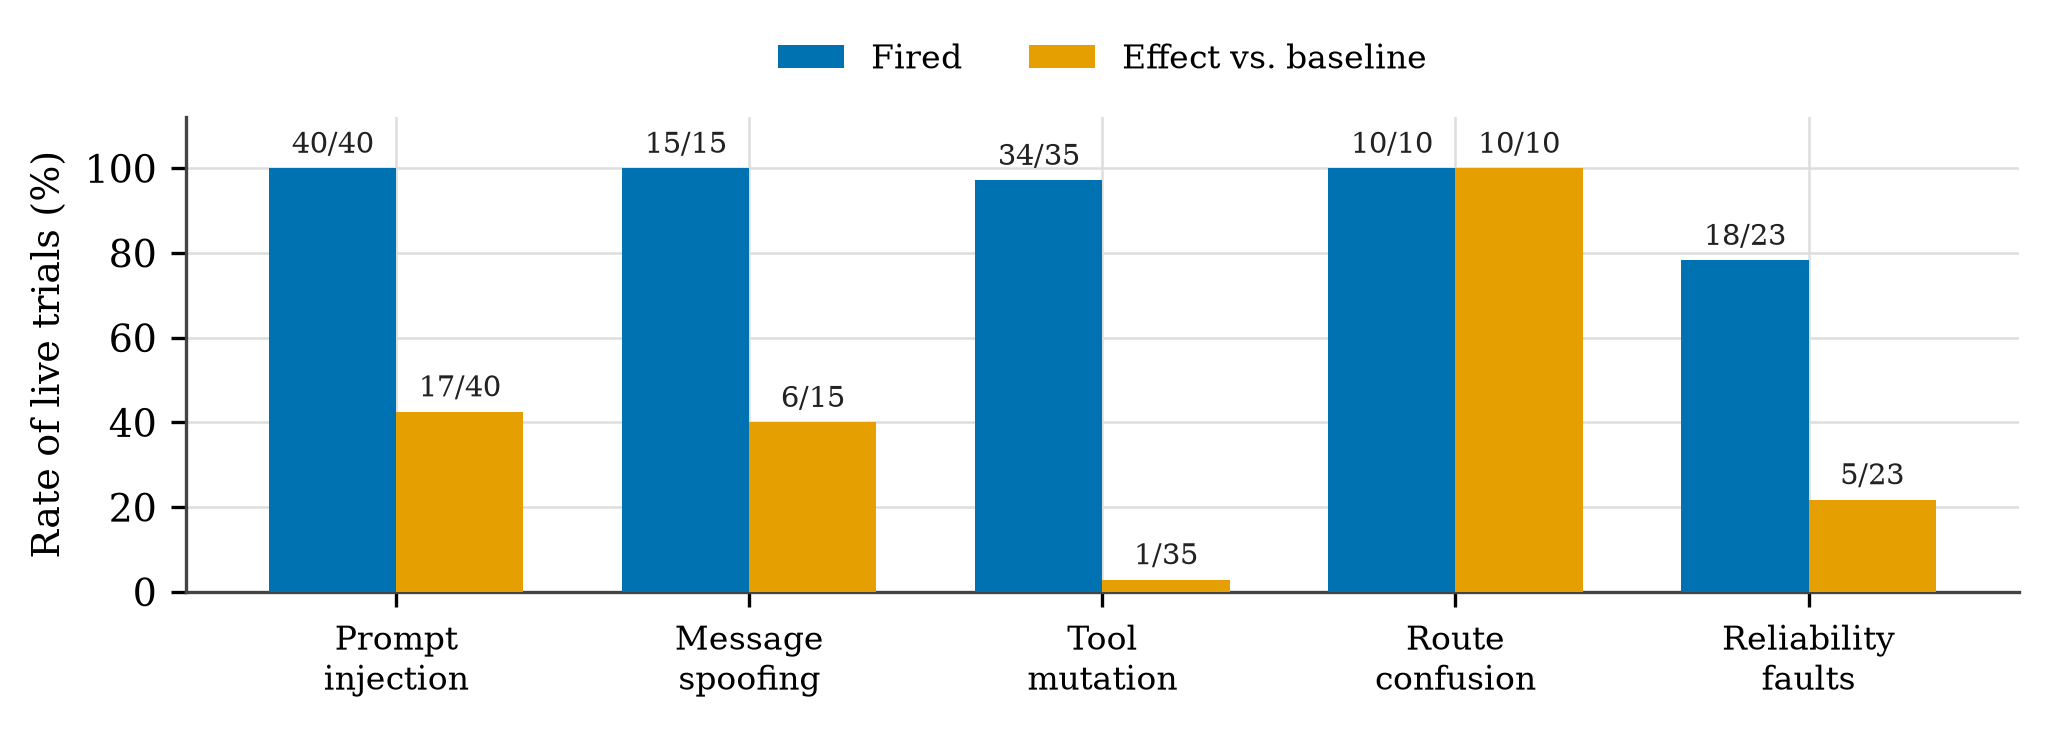
\includegraphics[width=\columnwidth]{figures/chart_attack_library.png}
\caption{The extended attack library's live trial outcomes by family (Section~\ref{sec:workloads}). Nearly every family fires close to 100\% of the time; whether that translates into a ground-truth-detected effect varies sharply -- route confusion is unambiguous and total, while prompt injection, message spoofing, and tool mutation show the model/backend resisting most attempts.}
\label{fig:library-chart}
\end{figure}

\section{Defenses: Security Mechanism Plugins and Zero Trust}
\label{sec:defenses}

Six security-mechanism plugins now cover every category a defense-in-depth testbed should, each registered through the identical \texttt{apply(ctx) -> HookResult} contract an attack plugin uses and classified in the trace as a distinct \texttt{POLICY\_EVENT} rather than misclassified as an attack. \textbf{\texttt{AmountLimitGuardrailPlugin}} denies a tool call whose declared amount exceeds a configured limit; live-verified blocking a tool-mutation attack that inflated a transfer from \$125.50 to \$5{,}000 before it reached the banking backend. \textbf{\texttt{RiskAwareRoutingGuardPlugin}} independently re-fetches a transaction's real risk score from the banking backend rather than trusting the router's own decision, closing route confusion -- the one attack that succeeded 5/5 undefended -- live-verified 5/5 deny and, with an optional \texttt{redirect\_to} recovery mode, 5/5 reaching the identical \texttt{manual\_review} ground truth the undefended baseline itself asserts. \textbf{\texttt{ResponseRedactionPlugin}} masks account-number-shaped tokens at the output control point; live verification surfaced and fixed a genuine Unicode-hyphen gap in its own detection regex. \textbf{\texttt{BatchIntegrityGuardPlugin}} closes the back office's own undefended ledger-mutation attack by independently re-checking a target batch's real expected-vs-posted totals, live-verified 5/5 with a control run confirming no false positive on the legitimate flow. \textbf{\texttt{RateLimitGuardrailPlugin}} caps calls per run/window/argument value, turning a hijack-induced crash (0/10 undefended) into 5/5 completed runs. \textbf{\texttt{ActionIsolationPlugin}} refuses tools with a chosen side effect regardless of caller, denying an attacked funds transfer in 5/5 trials with the backend's transaction count unchanged.

\textbf{Zero Trust Backplane.} MANTIS integrates the real, independently-developed \texttt{Citi\_P3\_Zero\_Trust\_Backplane} project's Task 4 signed Policy Decision Point~\cite{ztb_repo} -- not a reimplementation -- as a toggleable extension. A stock install never imports it; \texttt{zero\_trust\_enforcement} registers in the same plugin registry every other defense uses, guarded by a single \texttt{try/except ImportError}, so the optional dependency's absence means the plugin is genuinely unregistered rather than registered-but-broken. A dedicated \texttt{zero\_trust: \{enabled: true, pdp\_url: ...\}} block (or the equivalent checkbox in the minimal UI) turns it on or off per run; MANTIS's own contribution is \texttt{extensions/zero\_trust/generate\_policy.py}, which reads the testbed's live inventory and emits a default-deny-by-domain policy (an agent may act on a tool in its own domain; anything else is denied by the PDP's own default) in the real project's schema. Live verification confirmed same-domain allow, cross-domain deny, an unrecognized agent denied before a challenge is even issued, a shared tool name (\texttt{search\_policies}, front and mid office) resolving correctly in both directions, and two full legitimate workflow runs through the real PDP completing identically to the undefended baseline. Eleven regression tests guard this integration against future drift, verified by deliberately injecting two kinds of drift and confirming both were caught before reverting. This paper's own AML office (Section~\ref{sec:aml}) is registered in the same domain inventory this policy generator reads from, so the generated policy now also covers a fourth domain without any change to the generator itself.

\section{The AML Office: Porting Anti-Money Laundering from Citi\_P3}
\label{sec:aml}

\subsection{Motivation and Scope}

MANTIS's banking agents were extracted from a larger legacy monorepo, \texttt{Citi\_P3}~\cite{citi_p3_repo}, during the original migration documented in \texttt{MIGRATION.md}. That legacy codebase's \texttt{citi\_banking\_adk} package included a working AML investigation office -- an investigator agent, a SAR drafting agent, and four real detection functions -- that was never carried over when the rest of the codebase was translated into MANTIS's modular, hook-bus-instrumented architecture. This section reports that port: the detection logic is adapted, not reinvented, with the mathematics and control flow of every detection function unchanged from the source; MANTIS-side work is confined to the toggle mechanism, the agent-tree wiring, and the data-access layer the ported functions call into.

\subsection{Detection Logic}

Four detection functions are ported with their logic unchanged. \textbf{Structuring detection} (\texttt{detect\_structuring}) evaluates a sliding window over a customer's inbound deposit-like transactions (by transaction type or by destination-in-customer-accounts/source-not-in-customer-accounts), accumulating a rolling total and reporting a hit whenever that total, within a configurable window (default 7 days), meets or exceeds a configurable threshold (default \$10{,}000); a genuine hit creates a persisted AML alert and, optionally, a manual review case. \textbf{Threshold-anomaly checking} (\texttt{check\_threshold\_anomaly}) flags a transaction exceeding 5$\times$ a customer's baseline peak transfer amount. \textbf{Mule-ring detection} (\texttt{find\_mule\_rings\_for\_customer}) builds a directed graph from a customer's own transaction flows and reports closed loops via graph cycle detection, scoped -- as in the source -- to ring segments where the customer's own accounts appear as an endpoint. \textbf{Identity-document verification} (\texttt{verify\_identity\_document}) scores a submitted name (Unicode-normalized, case-folded, Levenshtein similarity), date of birth (exact calendar-date match), and ID number (exact string match) against reference values, weighted 0.30/0.30/0.40, returning a bounded, deterministic confidence score. Separately, an alert-lifecycle state machine (\texttt{open} $\rightarrow$ \texttt{in-investigation} $\rightarrow$ \texttt{cleared}/\texttt{escalated-to-sar}) is ported from the legacy codebase's standalone backend service into \texttt{BankingRepository}, the same SQLite-backed data-access layer every other banking tool already uses, with three new tool wrappers (\texttt{get\_aml\_alert}, \texttt{list\_aml\_alerts}, \texttt{transition\_aml\_alert\_status}) giving an agent a real path to use it.

\subsection{Toggle and Packaging}

The AML office follows the same two-layer toggle discipline Section~\ref{sec:defenses} established for Zero Trust, adapted to a domain rather than a policy plugin. \textbf{Per-run}: a dedicated \texttt{aml\_office: \{enabled: true\}} configuration block (mirroring \texttt{zero\_trust:}'s shape) controls whether the root agent's \texttt{sub\_agents} list includes the AML office router; every configuration without that block produces a root agent whose \texttt{sub\_agents}, instruction, and description are byte-identical to before this domain existed, verified directly by a regression test constructing the agent tree both ways and diffing it. \textbf{Packaging}: mule-ring detection's graph-cycle dependency (\texttt{networkx}) is an optional extra (\texttt{pip install -e ".[aml]"}), imported lazily inside the one function that needs it, so every other AML tool, and \texttt{mantis --inventory}/\texttt{--validate}, work in a stock install; calling the mule-ring tool without the dependency raises a clear, actionable \texttt{ImportError} rather than failing silently or crashing tool discovery.

\subsection{Live Verification: Two Real Defects Found and Fixed}
\label{sec:aml-verification}

Five scenarios exercise the AML office end to end against the live backend and a real model (\texttt{gpt-oss-20b} via UF Navigator): a structuring-detection positive case (three seeded inbound wires from one counterparty summing to \$12{,}000 within seven days, past the \$10{,}000 threshold), a structuring negative control, a mule-ring negative control, an identity-verification case, and an alert-triage case against a seeded reference alert. The first live pass of all five surfaced two real integration defects, neither caught by the unit test suite because both are properties of the \emph{live agent tree}, not of the ported functions in isolation -- the same class of finding both prior papers report as their central methodological lesson, that a clean exit or a passing unit test does not establish that a capability is reachable in the actual running system.

\textbf{Routing gap.} The identity-verification scenario was misrouted to \texttt{front\_office\_router} instead of \texttt{aml\_office\_router}: the root agent's routing instruction mentioned ``AML investigation, suspicious activity, and SAR drafting'' but not identity verification by name, and a plausible-sounding KYC-flavored prompt was reasonably routed to the front office instead, where it called \texttt{get\_customer\_context} with the submitted ID number in place of a customer id and produced a nonsensical result. The fix was wording, not logic: the root agent's and the AML router's instructions now explicitly name identity-document verification and alert triage as AML-office tasks.

\textbf{Unreachable capability.} The alert-triage scenario asked to transition a seeded alert's status; \texttt{transition\_aml\_alert\_status} existed, was correctly implemented, and was unit-tested directly as a function -- but no agent in the built tree had it, or its sibling read tools, on its toolset at all. The three alert-lifecycle tools were wired into the existing \texttt{aml\_investigator} agent's toolset, the single tool-using agent in this domain, and its instruction extended to describe the triage capability.

Both fixes verified live after correction: the identity-verification scenario now routes correctly to \texttt{aml\_office\_router} $\rightarrow$ \texttt{aml\_investigation\_workflow}, calls \texttt{verify\_identity\_document} with the exact submitted/reference values from the prompt, and reports 100\% match confidence. The alert-triage scenario now calls \texttt{transition\_aml\_alert\_status}, and we confirmed the effect directly against the database rather than trusting the model's own report: reading the alert back afterward shows its status genuinely changed from \texttt{open} to \texttt{in-investigation}. All five scenarios were then run officially from committed configuration files (\texttt{configs/extensions/aml\_office\_*\_demo.yaml}) and scored by \texttt{mantis --evaluate}: \texttt{tool\_use\_correctness} 1.0 and \texttt{workflow\_outcome} 1.0 (\texttt{completed}) for every one of the five, with zero missing expected tools and zero forbidden tools used. Table~\ref{tab:aml-live} summarizes all five after both fixes.

\begin{figure}[t]
\centering
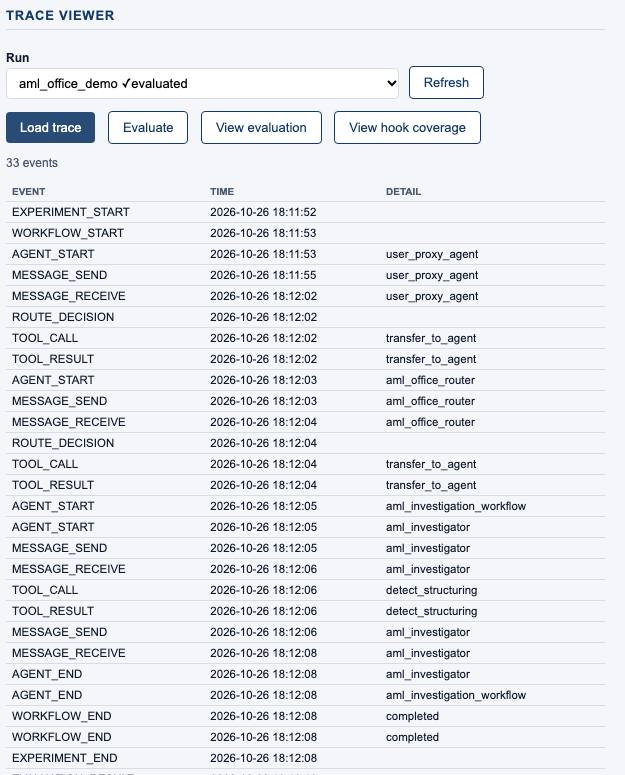
\includegraphics[width=\columnwidth]{figures/ui_trace_crop.png}
\caption{The minimal UI's Trace Viewer (Section~\ref{sec:workloads}) rendering the real \texttt{aml\_office\_demo} trace -- every event is real, from this run, not illustrative: the root agent's two \texttt{transfer\_to\_agent} hops into the AML office, then \texttt{aml\_investigator}'s own \texttt{detect\_structuring} call and result.}
\label{fig:ui-trace}
\end{figure}

\begin{figure}[t]
\centering
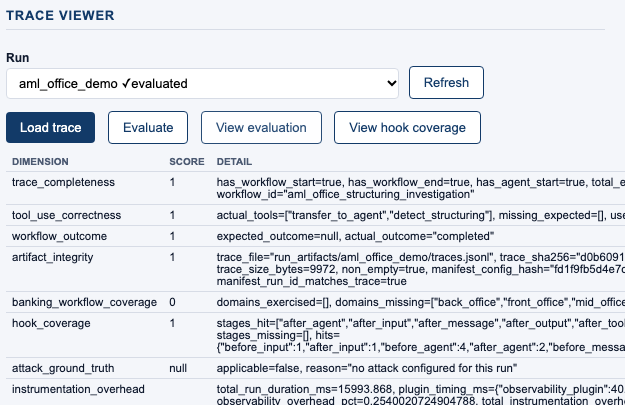
\includegraphics[width=\columnwidth]{figures/ui_eval_crop.png}
\caption{The same UI, scoring the same run: \texttt{tool\_use\_correctness} and \texttt{workflow\_outcome} both 1.0, matching the \texttt{mantis --evaluate} CLI output reported above exactly, since both call the identical evaluator -- the UI has no separate scoring logic of its own. \texttt{banking\_workflow\_coverage} is 0 here, correctly: an AML-office-only run exercises none of the other three domains.}
\label{fig:ui-eval}
\end{figure}

\begin{table}[t]
\centering
\caption{AML office live verification, all five scenarios, against a real model after the fixes in \S~\ref{sec:aml-verification}.}
\label{tab:aml-live}
\scriptsize
\begin{tabular}{@{}p{2.3cm}p{1.0cm}p{4.0cm}@{}}
\toprule
Scenario & Tool called & Observed \\
\midrule
Structuring (positive) & \texttt{detect\_\allowbreak structuring} & Correctly detected \$12{,}000 cumulative over 7 days; real alert and manual-review case persisted. \\
Structuring (routine control) & \texttt{detect\_\allowbreak structuring} & Correctly reported no structuring; no alert created. \\
Mule ring (control) & \texttt{find\_mule\_\allowbreak rings\_for\_\allowbreak customer} & Correctly reported no closed loop in the seeded history. \\
Identity verification & \texttt{verify\_\allowbreak identity\_\allowbreak document} & Correctly routed after fix; 100\% match confidence on identical submitted/reference values. \\
Alert triage & \texttt{transition\_\allowbreak aml\_alert\_\allowbreak status} & Correctly routed after fix; database re-read confirms the real status transition. \\
\bottomrule
\end{tabular}
\end{table}

\subsection{An Honest Limitation Inherited, Not Introduced}

The ported \texttt{detect\_structuring} function is deterministic and, as Table~\ref{tab:aml-live} shows, correct. The \emph{investigator agent's} own judgment on top of a correct detection is an LLM call, and its gating logic for whether to draft a SAR (risk score $\geq$ 50, or an investigation status containing ``suspicious'') is inherited unchanged from the source prompt. A live run against the positive structuring case correctly identified the pattern in its \texttt{findings} text but assigned a risk score of 7.2 -- well under the reporter's trigger threshold -- and, separately, populated its \texttt{case\_facts} with invented transaction amounts and dates rather than the real values the tool had just returned. We report this as a known limitation of that prompt against this specific smaller model, inherited directly from \texttt{Citi\_P3} and not something this port introduced or silently corrected, consistent with both prior papers' practice of reporting a defense's real scope rather than overstating it.

\section{Additional Workloads, UI, and Scenario Library}
\label{sec:workloads}

Three additional banking workloads, each backed by real persisted records rather than a new prompt into an existing process: dispute filing (front office), SAR/exception escalation (back office), and loan pre-approval (mid office), the last computing a real, deterministic decision from seeded account data rather than an LLM opinion. A second institution profile (\texttt{regional\_credit\_union}) reuses every agent, tool, and workflow unchanged against an isolated database and a genuinely stricter policy threshold (10\% of balance versus 25\%), selected by a runtime configuration field. A minimal, schema-driven browser UI (\texttt{mantis --ui}) provides an experiment editor and trace viewer whose every mutating action -- validate, run, campaign -- shells out to the identical \texttt{mantis} CLI subprocess a terminal user would invoke, verified by confirming a deliberately invalid configuration returns the real CLI's own error text rather than a UI-side check; dedicated toggle fieldsets for Zero Trust and the AML office sit alongside the generic attack/policy dropdowns. An extended scenario library ships 19 measured no-attack baselines and 26 attack/fault variants (123 scored live trials across five families), and a from-scratch walkthrough adding a new attack plugin in about fifteen lines. Five starter campaigns -- the original four~\cite{mantis_paper2} plus a fifth added for this paper's own AML office, sweeping its five scenarios with no attack configured and live-verified at \texttt{tool\_use\_correctness} 1.0 across all five -- each a single \texttt{mantis --campaign} command producing a consolidated report. The AML office extends the scenario library by five further scenarios under its own domain (Section~\ref{sec:aml}), each reproducible from a committed configuration file.

\section{Evaluation Summary}
\label{sec:evaluation}

The offline test suite -- unit and contract tests, a parametrized consistency suite over every shipped configuration and scenario, and regression guards for every toggleable extension -- stands at 853 passing tests with neither optional dependency (\texttt{zero\_trust}, \texttt{aml}) installed, 880 with both installed, zero failures in every combination, and 178 more skipped by design without a live backend or model. This paper's own AML office extension adds 53 of those tests (repository-layer, detection-function, toggle, and drift-regression coverage) on top of the base established by~\cite{mantis_paper1} and the fourteen further categories added by~\cite{mantis_paper2}. Table~\ref{tab:complete-evidence} consolidates live-verification evidence across the complete system.

\begin{table}[t]
\centering
\caption{Complete-system live-verification evidence.}
\label{tab:complete-evidence}
\scriptsize
\begin{tabular}{@{}p{2.1cm}p{5.2cm}@{}}
\toprule
Capability & Live evidence \\
\midrule
Attacks/failures (5) & Route confusion 5/5 fired+effect; tool mutation genuinely reaches and alters the real call every trial; prompt injection, message spoofing, malformed-failure control genuinely reach the model/agent 5/5 with the agent correctly resisting each. \\
Defenses (6) & Every attack that once succeeded 5/5 undefended now has a live-verified 5/5 defense; no false positive on any paired no-attack control. \\
Zero Trust Backplane & Same-domain allow, cross-domain deny, unrecognized-agent pre-challenge deny, two full legitimate runs through the real PDP identical to baseline. \\
AML office (new) & All 5 scenarios correct after fixing 2 real integration defects found via live verification (Table~\ref{tab:aml-live}); one transition confirmed against the database, not just the model's report. \\
Additional workloads (3) & Live, 5/5 each: real persisted dispute, SAR, and loan-decision records. \\
Institution variant & Live, 5/5: identical code path, isolated data, genuinely different real decision. \\
Minimal UI & Real invalid config rejected with the real CLI's own error text; real server confirmed via HTTP. \\
Scenario library & 123 scored live trials across 26 attack/fault variants; 5 more for the AML office. \\
\bottomrule
\end{tabular}
\end{table}

\section{Conclusion}
\label{sec:conclusion}

This paper consolidates MANTIS as a complete system: the original five-control-point testbed~\cite{mantis_paper1}, all five of its deferred extensions~\cite{mantis_paper2} including a real, toggleable Zero Trust Backplane integration, and -- new here -- a toggleable AML office porting real structuring, mule-ring, and identity-verification detection logic from the legacy \texttt{Citi\_P3} codebase MANTIS was originally extracted from. Every extension across all three papers shares the same discipline: a capability is reported as working only once verified against the system's actual emitted trace or persisted database state, not a clean exit code or a passing unit test in isolation. The AML office extension is itself a fresh instance of that discipline's value: live verification against five new scenarios found two real defects -- a routing-instruction gap and an unreachable, unwired tool capability -- that no unit test caught, because both are properties of the live agent tree rather than of any single ported function, and both were fixed and re-verified, including one effect confirmed directly against the database rather than accepted from the model's own report. The complete offline suite passes with zero failures across all four combinations of its two optional dependencies (853 with neither, 880 with both), and every live capability this paper reports -- attacks, defenses, Zero Trust, the three additional workloads, the institution variant, the UI, and now the AML office -- is reproducible from a committed configuration file against the real backend and a real model, consistent with the evidentiary standard both prior papers set for themselves.

\section*{Acknowledgment}
% Insert acknowledgment of funding sources and individual contributions here.

\begin{thebibliography}{00}

\bibitem{mantis_paper1}
[Authors], ``MANTIS -- Modular Agent Network Testbed for Instrumentation and Security in Multi-Agent Banking Systems,'' 2026.

\bibitem{mantis_paper2}
[Authors], ``MANTIS Extended -- Post-Paper Extensions to a Banking Multi-Agent Security Testbed,'' 2026.

\bibitem{citi_p3_repo}
smartsystemslab-uf, ``Citi P3,'' \texttt{github.com/smartsystemslab-uf/Citi\_P3}, 2026. (Legacy source repository MANTIS's banking agents were extracted from.)

\bibitem{ztb_repo}
smartsystemslab-uf, ``Citi P3 Zero Trust Backplane,'' \texttt{github.com/smartsystemslab-uf/Citi\_P3\_Zero\_Trust\_Backplane}, 2026.

\bibitem{anomaly_detection_finance}
X.~Zhang et al., ``Enhancing Anomaly Detection in Financial Markets with an LLM-based Multi-Agent Framework,'' \emph{arXiv preprint arXiv:2403.19735}, 2024.

\bibitem{masca_credit}
``MASCA: LLM based-Multi Agents System for Credit Assessment,'' \emph{arXiv preprint arXiv:2507.22758}, 2025.

\bibitem{prompt_infection}
D.~Lee and M.~Tiwari, ``Prompt Infection: LLM-to-LLM Prompt Injection within Multi-Agent Systems,'' \emph{arXiv preprint arXiv:2410.07283}, 2024.

\bibitem{aitm_communication_attacks}
``Red-Teaming LLM Multi-Agent Systems via Communication Attacks,'' in \emph{Findings of the Association for Computational Linguistics: ACL 2025}, arXiv preprint arXiv:2502.14847.

\bibitem{agentic_security_survey}
``A Survey on Agentic Security: Applications, Threats and Defenses,'' \emph{arXiv preprint arXiv:2510.06445}, 2025.

\bibitem{security_considerations_mas}
``Security Considerations for Multi-agent Systems,'' \emph{arXiv preprint arXiv:2603.09002}, 2026.

\bibitem{redagentbench}
``REDAgentBench: Executable Red Teaming and Faithful Measurement of LLM Agent Systems,'' \emph{arXiv preprint arXiv:2608.10669}, 2026.

\bibitem{nist_zero_trust}
S.~Rose, O.~Borchert, S.~Mitchell, and S.~Connelly, ``Zero Trust Architecture,'' NIST Special Publication 800-207, National Institute of Standards and Technology, Aug. 2020.

\bibitem{zero_trust_agentic_identity}
``A Novel Zero-Trust Identity Framework for Agentic AI: Decentralized Authentication and Fine-Grained Access Control,'' \emph{arXiv preprint arXiv:2505.19301}, 2025.

\end{thebibliography}
\vspace{12pt}

\end{document}
